
\chapter{Appendix}
\begin{figure}[ht]
       \centering 
	    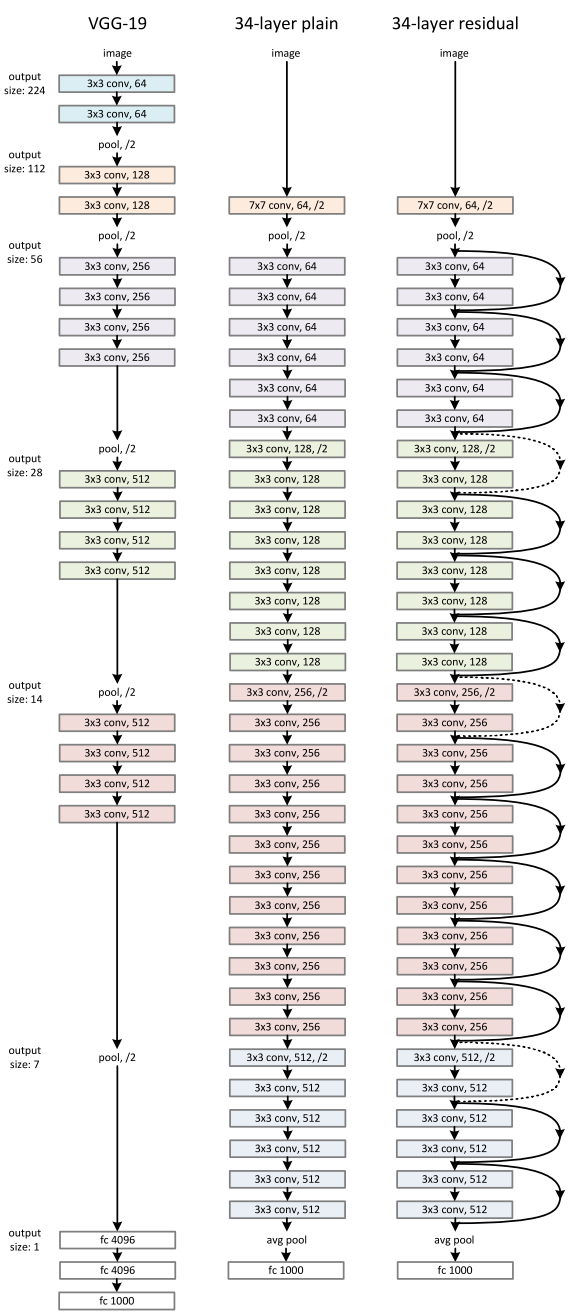
\includegraphics[width = 10 cm]{resnet_arch_full.png}
        \caption[Example of the architecture of residual networks]{ Left: the VGG-19 model [41] (19.6 billion FLOPs) as a reference. Middle: a plain network with 34 parameter layers (3.6 billion FLOPs). Right: a residual network with 34 parameter layers (3.6 billion FLOPs). The dotted shortcuts increase dimensions.\cite{DBLP:journals/corr/HeZRS15}}
         \label{fig:resnet_arch_full}
\end{figure}
\begin{figure}[ht]
       \centering 
	    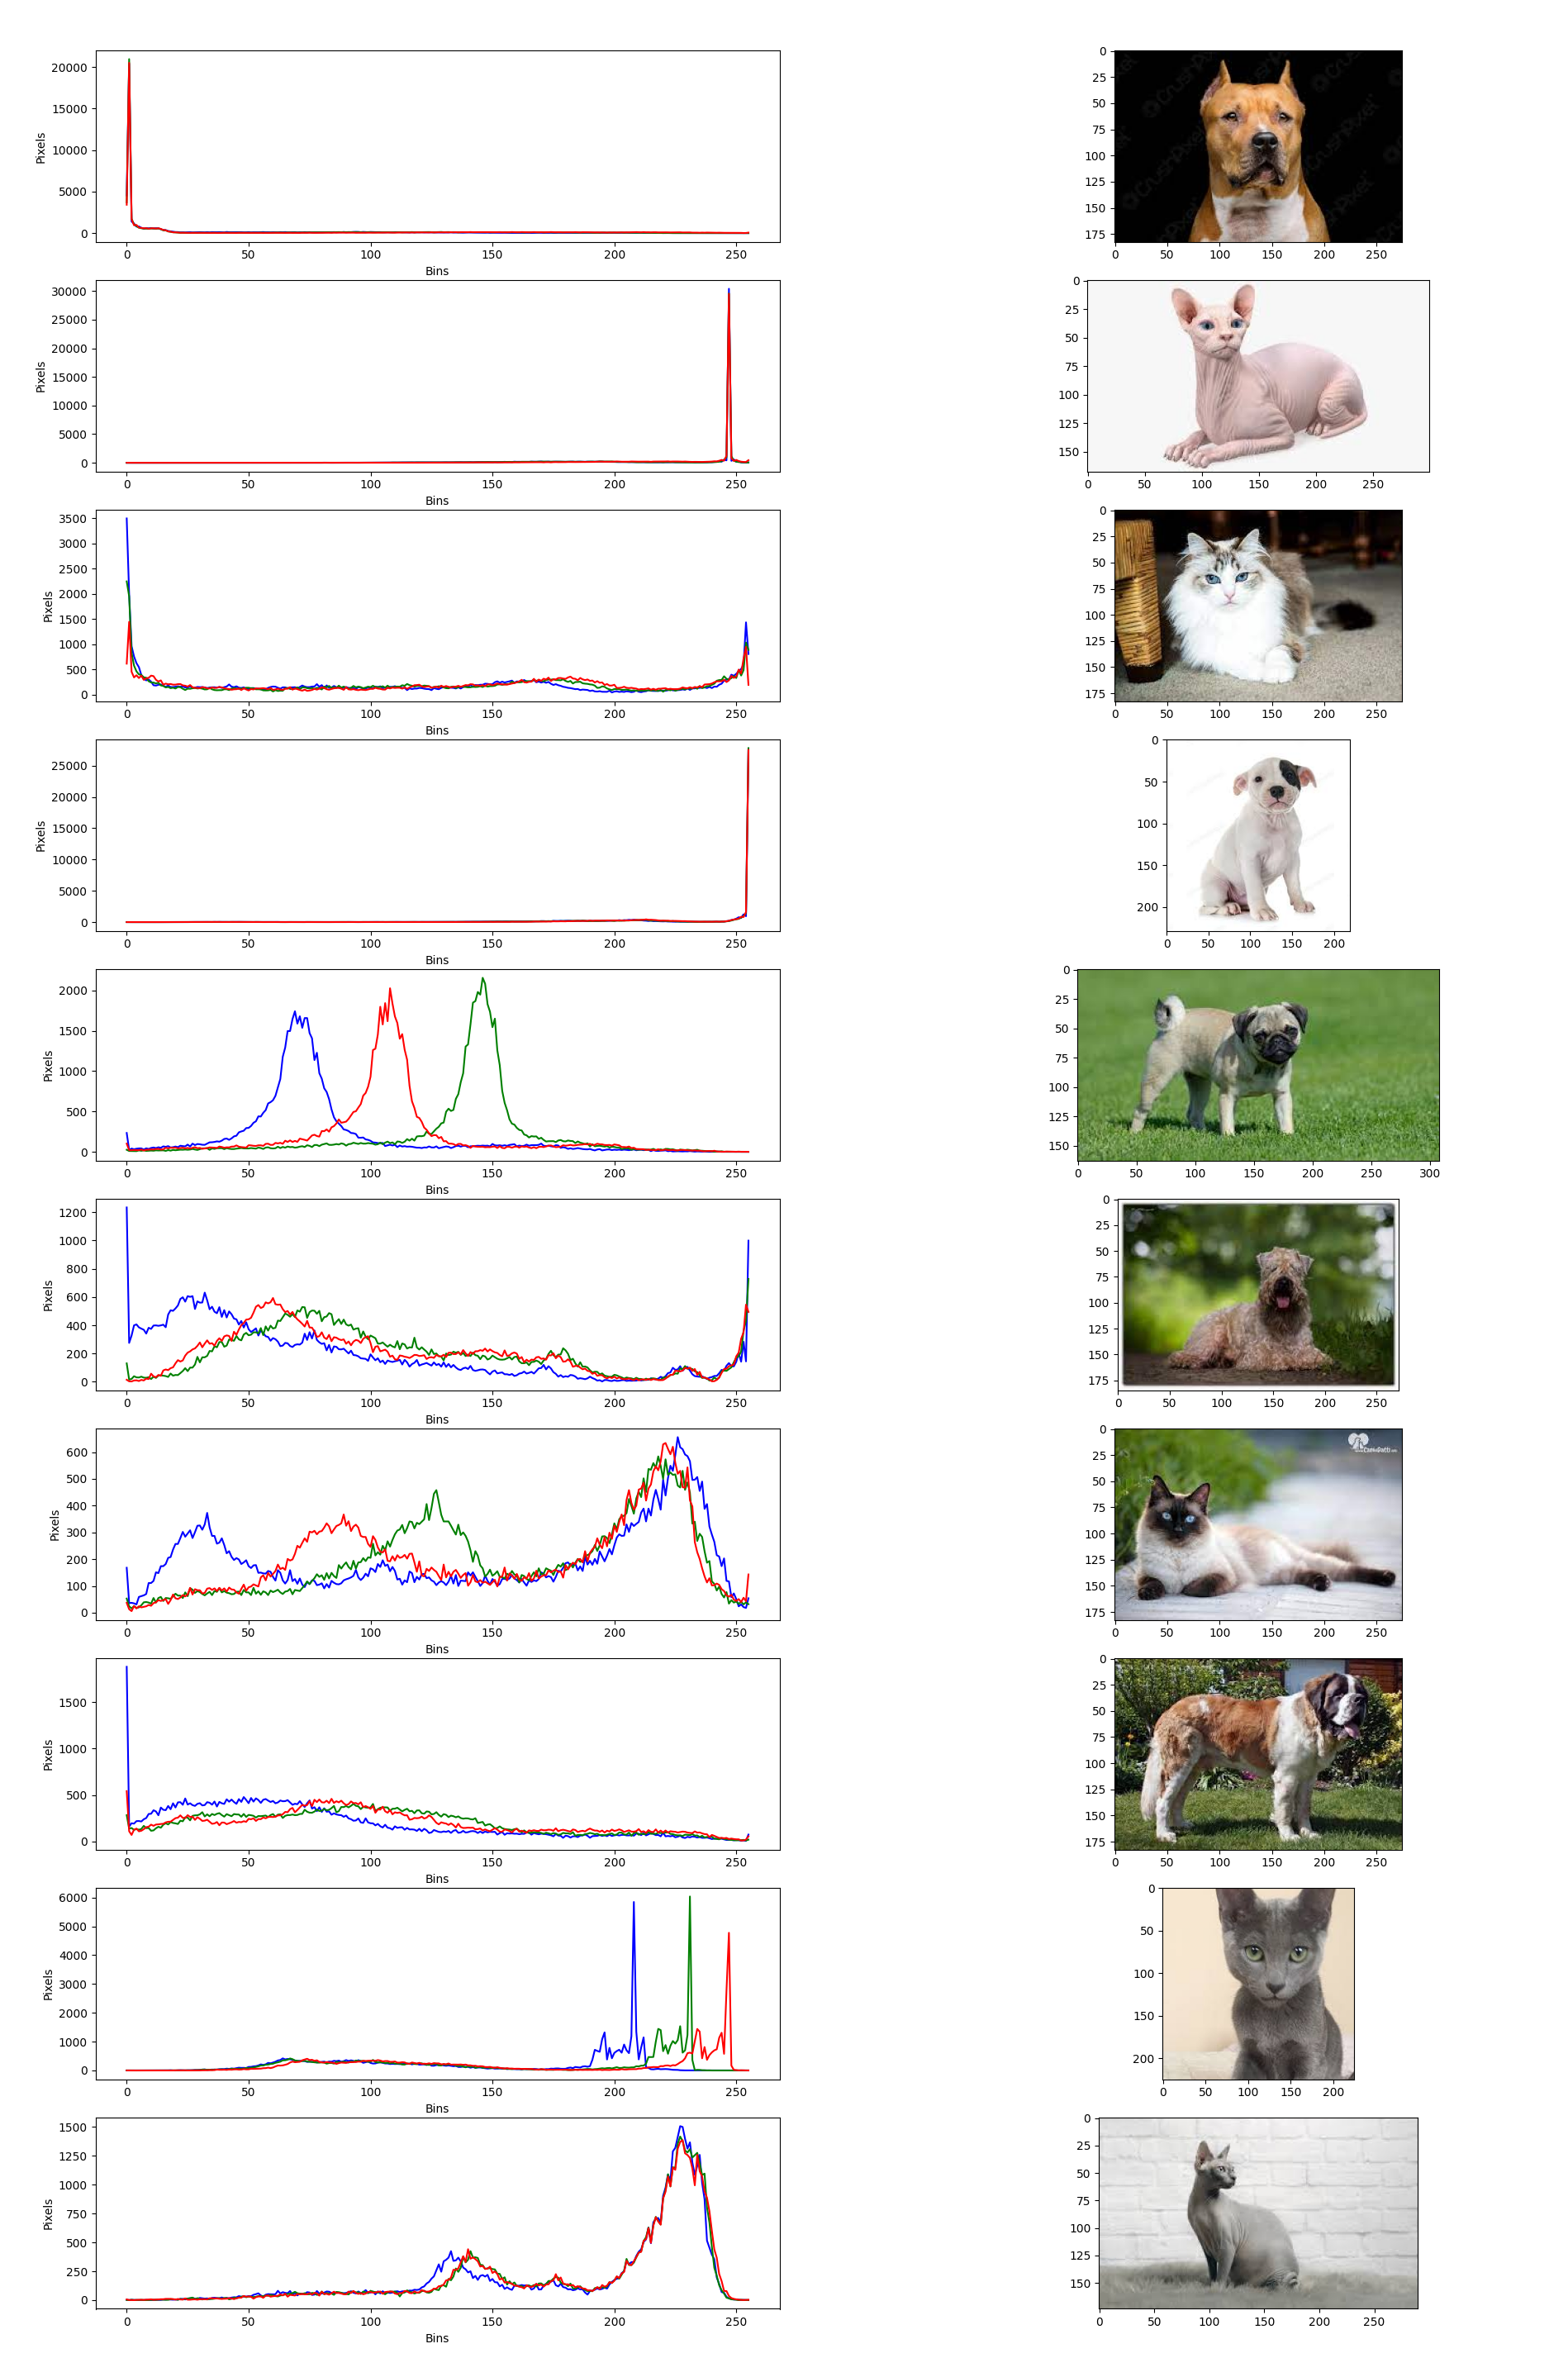
\includegraphics[width = 13 cm]{fastest_files.png}
        \caption{Histogram of the fastest files}
         \label{fig:fastest_files_his}
\end{figure}

\begin{figure}[ht]
       \centering 
	    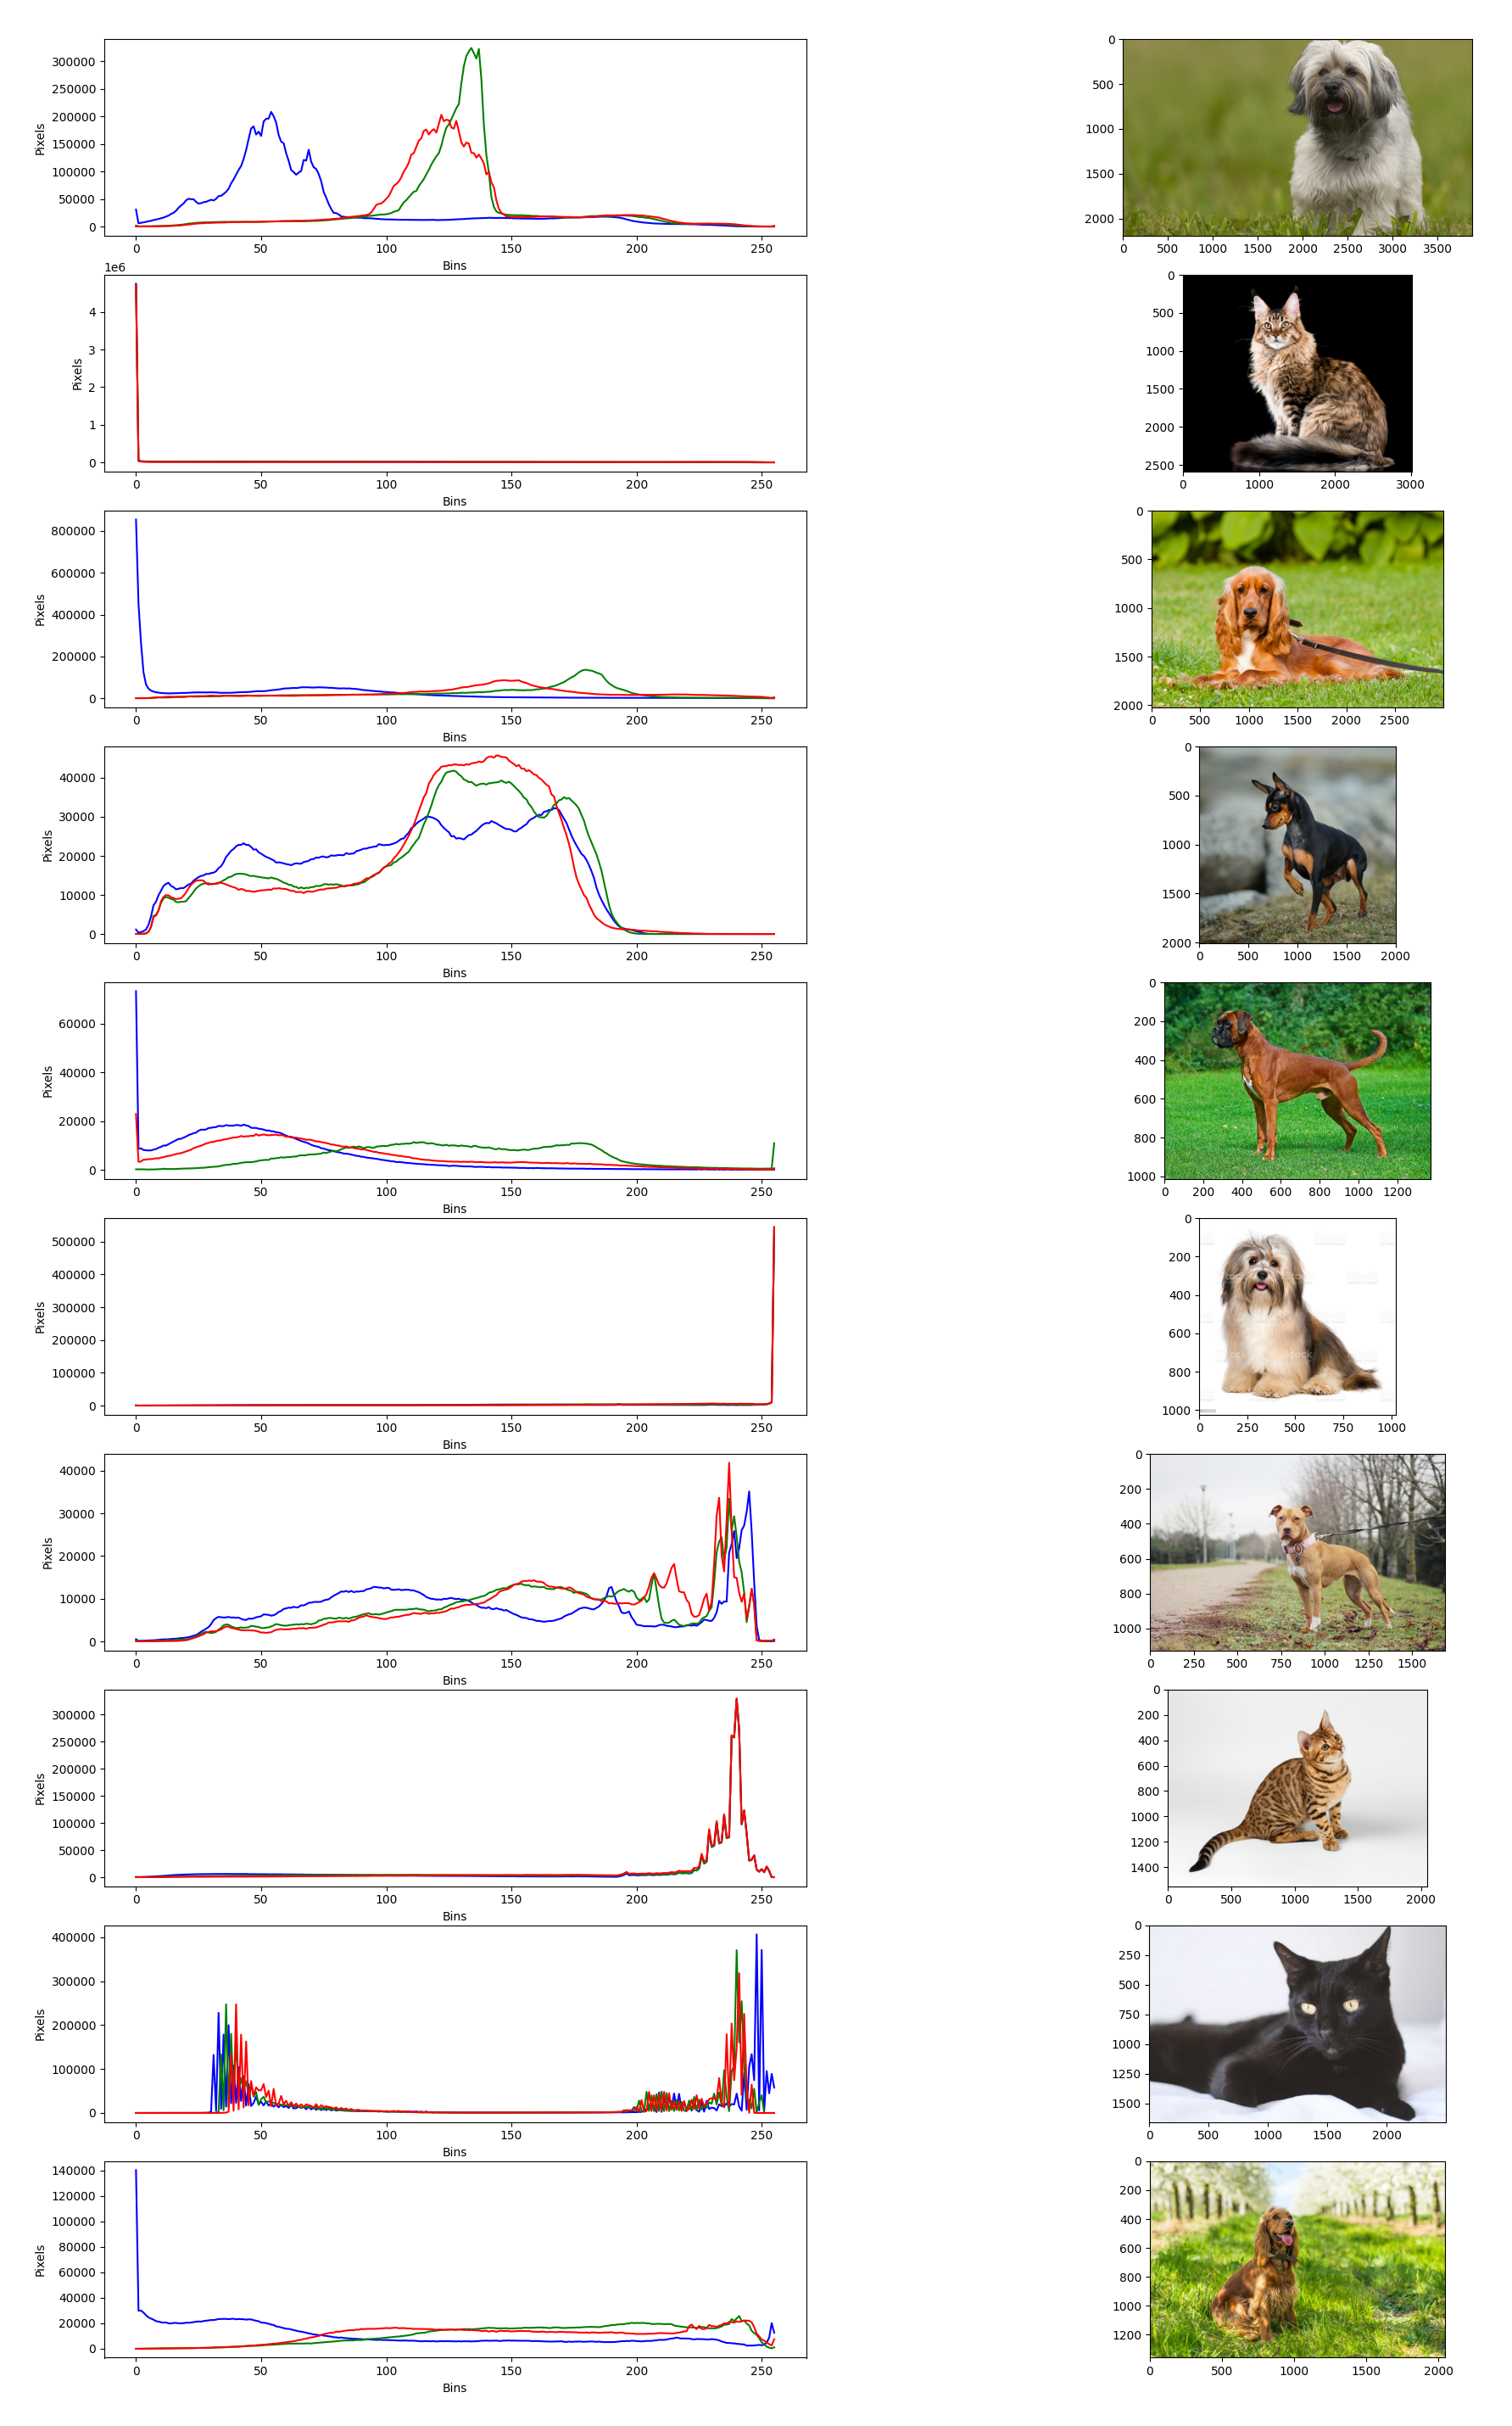
\includegraphics[width = 13 cm]{slowest_files.png}
        \caption{Histogram of the slowest files}
         \label{fig:slowest_files_his}
\end{figure}



